\documentclass{standalone}

\usepackage{tikz}

\begin{document}
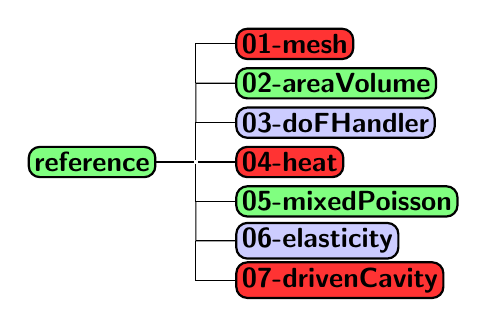
\begin{tikzpicture}
  
  \node[anchor=center,inner sep=-1mm] (X) at (0,0) {};

  % node styles
  \tikzstyle{Box}=[
  anchor=west,
  thick,
  font=\sffamily\bfseries,
  align=center,
  inner sep=0.7mm,
  shape=rectangle,rounded corners,draw]

  \tikzstyle{Label}=[font=\sffamily\bfseries\tiny]

  \draw (X) node[Box,anchor=east,fill=green!50] (I)  at +(-0.5,  0.0) {reference};

  \draw (X) node[Box,fill=  red!80] (A4)  at +(0.5, 1.5) {01-mesh};
  \draw (X) node[Box,fill=green!50] (A5)  at +(0.5, 1.0) {02-areaVolume};
  \draw (X) node[Box,fill= blue!20] (A6)  at +(0.5, 0.5) {03-doFHandler};

  \draw (X) node[Box,fill=  red!80] (A7)  at +(0.5, 0.0) {04-heat};

  \draw (X) node[Box,fill=green!50] (A8)  at +(0.5,-0.5) {05-mixedPoisson};
  \draw (X) node[Box,fill= blue!20] (A9)  at +(0.5,-1.0) {06-elasticity};
  \draw (X) node[Box,fill=  red!80] (A0)  at +(0.5,-1.5) {07-drivenCavity};

  \draw (I.east) -- (X);
  \draw (X) -- (A7.west);
  \draw (X) -- ++(0,-0.5) -- (A8.west);
  \draw (X) ++(0,-0.5) -- +(0,-0.5) -- (A9.west);
  \draw (X) ++(0,-1.0) -- +(0,-0.5) -- (A0.west);

  \draw (X) -- ++(0,0.5) -- (A6.west);
  \draw (X) ++(0,0.5) -- +(0,0.5) -- (A5.west);
  \draw (X) ++(0,1.0) -- +(0,0.5) -- (A4.west);

\end{tikzpicture}
\end{document}


%%% Local Variables: 
%%% mode: latex
%%% TeX-master: t
%%% End: 
